\section{Základní nelinearity a popis nelineárních systémů (popis statických a dynamických nelineárních systémů,
vliv parazitních nelinearit na průběh regulačního děje)}



\subsection{bez dynamiky}
Systém reaguje na odezvu okamžitě, nebo je jeho časová kosatanta výrazně nižší něž zyblé čas. konstanty.
Dělí se na :

\begin{itemize}
    \item bez paměti
    \item s pamětí
\end{itemize}

\subsubsection*{nelinearita bez paměti}

Dá se vyjádřit jako funkce 
\begin{equation}
    y=f(u)
\end{equation}

Na zákadě aktuální hodoty se určí výstup. Dá se jednoduše linearizovat rozvojem da taylorovy řady, nebo do polynomu.
posána funkcí, grafem, tabulkou.
\\
např. :  saturace, tření\dots
\\
\\
\subsubsection*{nelinearita z pamětí}
Výstup zálezí i na předchozích satvech, nelze jednoduše popsat jako funkce, často se popisuje slovně nebo jako algorytmus.
\\
např.: vůle v převodech, relé s hysterezí

\subsection*{Základní nelinearity}

\subsubsection*{nasycení(saturace)}
\begin{itemize}
    \item nejběžnejší nelinearita (obsahuje ji vpodstatě každý reálný systém)
    \item dá se s ní pracovat jako s po částech lineární funkcí
    \item pokud zajistíme že se systém nedosatne z <b,a> lze prát jako lin. f-ce 
    \item např.: nádrž co přeteče
    \item (je jedním z faktorů pro vzik wind up jevu)
    \item bez paměti
\end{itemize}
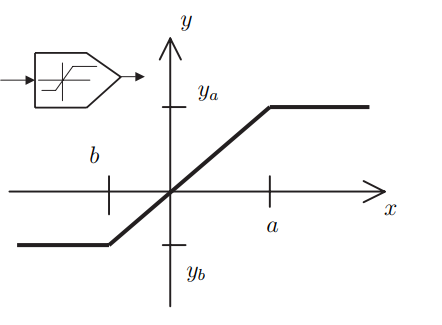
\includegraphics[]{img/saturace.png}

\subsubsection*{necitlivost}
\begin{itemize}
    \item nejčasttěji u mech systémů (projev tření a mech. nepřesností)
    \item např.: DC motor se roztočí až od určitého napětí
    \item občas se vkládá do reg. umělěle aby se omezili oscilace
    \item po částech lineární (většinou)
    \item bez paměti
\end{itemize}
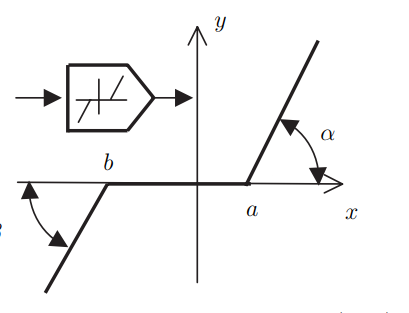
\includegraphics{img/necitlivost.png}

\subsubsection*{vůle v převodech (hystereze)}
\begin{itemize}
    \item při změně pohybu chíli trvá než se něco začne dít
    \item v převodovkách , nebo při magnetizaci železa (hysterezní symčka- v otázce MVE mag. měřemí)
    \item v převodovce lze odstarnit tak že druhý motor tlačí vždycky proti
    \item rádi se na to ptají
    \item vetšinou nelze linearizovat
    \item s pamětí
\end{itemize}
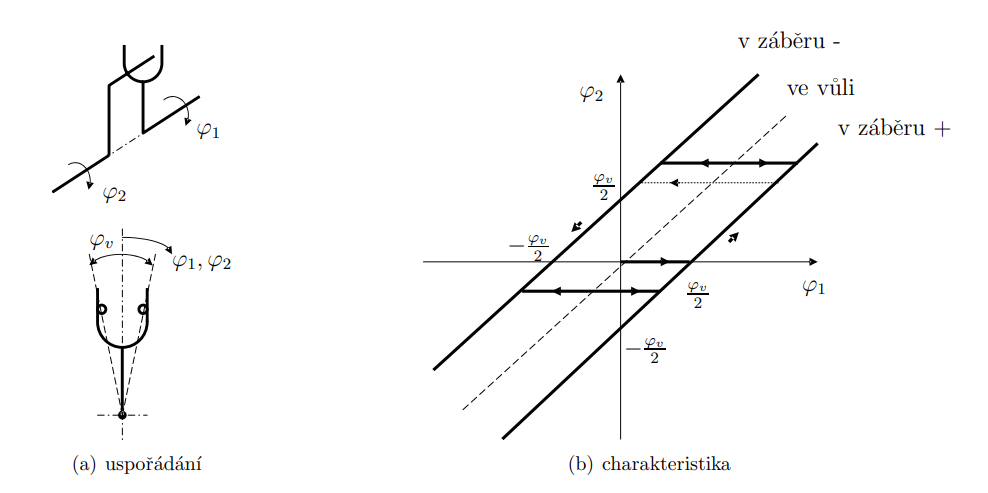
\includegraphics{img/vule.png}

\subsubsection*{tření}
\begin{itemize}
    \item v mech systémech
    \item špatně se linearizuje v oklí 0
    \item bez paměti
\end{itemize}
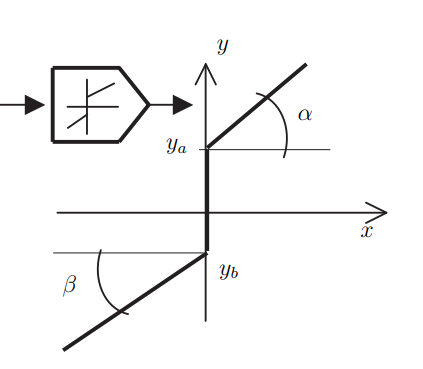
\includegraphics{img/treni.png}

\subsection*{releové charakteistiky}
\begin{itemize}
    \item s pamětí i bez
    \item požití jako regulátor
\end{itemize}
\includegraphics*{img/rele.png}


\subsection{s dynamikou}
popsány stavovými rovnicemi:
\[
    \frac{dx}{dt}=f(x,u)\]
    \[y=g(x,u)\]


\begin{itemize}   
    \item časově variantní
    \item časově invariantí (paramtry se v čase nemění)
\end{itemize}
%----------------------------------
\newpage
\section{Ustálené chování nelineárních dynamických systémů (rovnovážné stavy, mezní cyklus, metoda
harmonické rovnováhy, stabilita mezního cyklu)}

Není v otázce přímo zmíněný ale asi dobrý vědět.

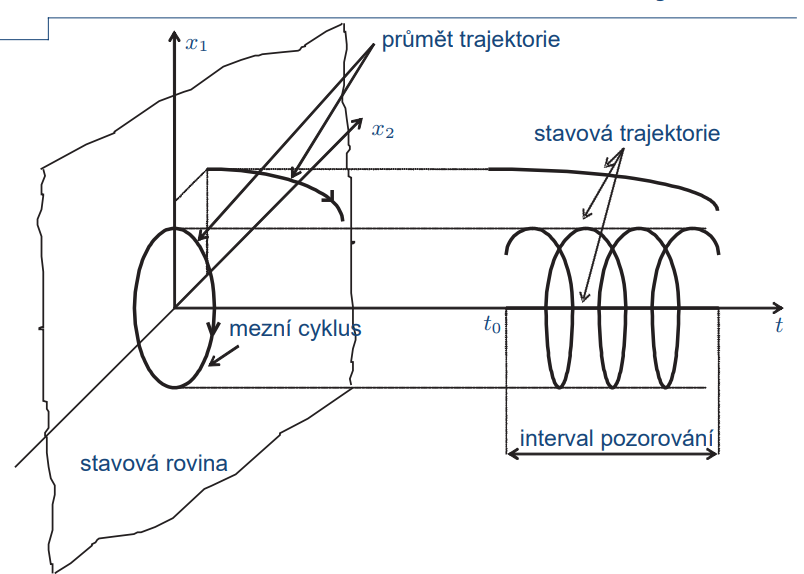
\includegraphics[scale = 0.8]{img/trajektorie.png}
{
\it stavová trejektorie (po systém 2. řádu) je 3d graf ukazuje jak se v čase mění vnitřní stavy systému.
Požívá se průmět stavové trajektorie, ukazuje jak se bude systém chovat, šipkou naznačeno odkuk kam se bude v čase pohyboavt.
}
\subsection{rovnovážný stav}
Stav systému, ktrý se v čase nemění. x=0 Průmět stavové trajekotrie je bod. Určíme
ho jako \[ \dot{x} = 0 \]
Systém může mít o vice rovnocážných stavů, také nemusí mít žádný.

Rovnovážné stavy mohu být:
\begin{itemize}
    \item izolované - pokud kolem něj exzistuje jeho maůlé okolí ve kterém se nenachází dlaší rovnovážný stav.
    \item neizolované
\end{itemize}

U rovnovážných stavů pak můžeme řešit jejich stbilitu pokud se systém po drobném vychýlení do rovanážného 
satvu vrátí je rovnovážný stav stabilní.
O stabilitě/nestabilitě lze rohodnou lineazizací rozvojem do taylorovy řady (podle polohy pólů náhrady)


\subsubsection{mezní cyklus}
Mezní ckyclus nastáva pokud se stavysystému pridicky opakují, průmět satv trajetorie je uazvřený obrazec (kruh).
Matematicky řečeno :
\[x(t+T)=x(t)\]
t-čas \\ T-perioda\\

Mezní cykus muže být stbiln polostabilní nebo nesatbilní:  


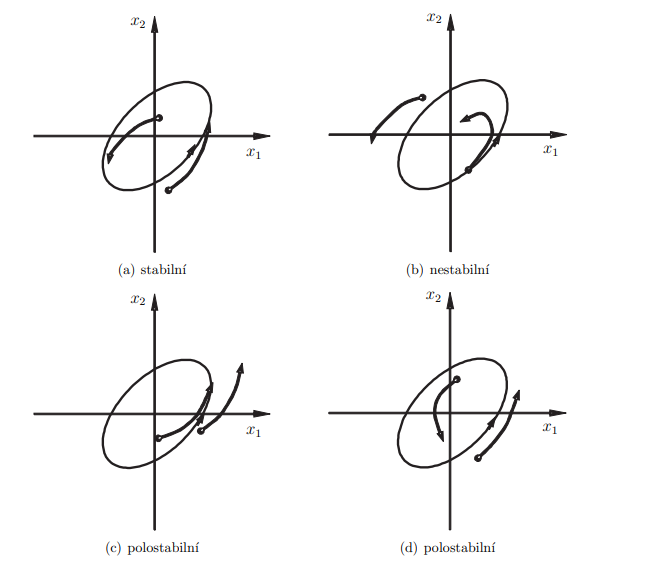
\includegraphics{img/mez_cykly.png}


Zda vrnikou mezní cykly jde určit metodou harmonické rovnováhy
\subsubsection*{metoda harmonické rovnováhy}
Vyžívá ekvivalentního opřenosu nelinearity ke zkoumání mezních cyklů.

\subsubsection*{ekvivaletní přenos}
nelinearitu nahradíme nahdíme ekvivaletním přenosem $N_e$, ten je závislá na AMplitudě vstupního signálu A.

Ekvivalenní přenos zsíkáme  tak, že odezvu nelinearity na harmonický průběh o amplitudě A, převdeme pomocí furierovy tranformace na jeho ekvivaletní přenos. U furierovy transformace uvažujeme pouze 1. harmonickou, 
protože se bere že další části obvodu mají charakter dolní propusti. Matematicky řečeno:
\begin{equation*}
    N_e= \frac{a_1+j\cdot b_1}{A}
\end{equation*}
kde
\begin{equation*}
    a_1=\frac{2}{T} \int_{0}^{T} f(e) \cdot sin(\omega t) dt
\end{equation*}

\begin{equation*}
    a_1=\frac{2}{T} \int_{0}^{T} f(e) \cdot cos(\omega t) dt
\end{equation*}

{\bf Tuto náhradu lze použít pouze pokud}
\begin{itemize}
    \item je dalším prvkem v regulačním obvodu systém typu doní propust, který dostatečně potlačuje vyšší harmonické
    \item nelinearita při vstupním signálu $e=A\cdot sin (\omega t) $ negeneruje stejnosměrnou složku
\end{itemize}



Zjištění mezních cyklů 


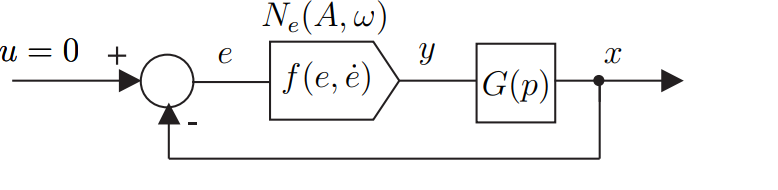
\includegraphics{img/harm.rovnovha.png}

Pro urční mezních cyhlů musý být systém jako je na obrázku, kde f je nelinearita a G je lin přenos typu dolní propust.

Mezní cykly v systému vzniknou pokud bude "$ F_o =-1 $", tedy pokud bude výstup systému 
roven jeho vytupu posuntému o 180°, matematicky :
\begin{equation*}
    A= N_e \cdot G \cdot A
\end{equation*}
Úpravou dostaneme podmínku vzniku mezních cyklů jako :
\begin{equation*}
    G=\frac{-1}{N_e}
\end{equation*}
Tato rovnice často nelze numericky řešit a musí se řešit garficky.

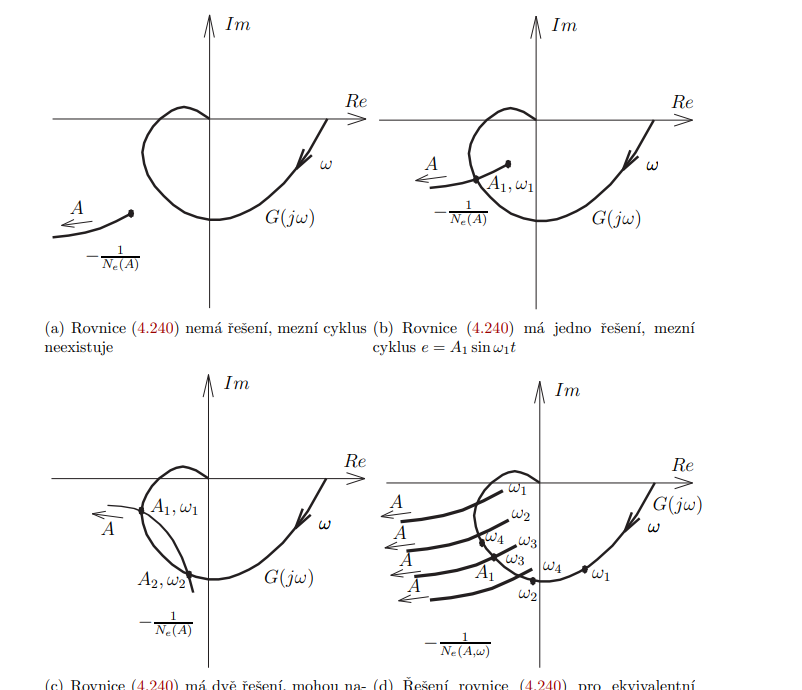
\includegraphics{img/garf.reseni.png}

dál lze touto metodou určit jeslti je mezní cyklus stabilní, pomocí modifikovaného Nyquistova kritéria :
 napříklda u bodu 1, pokud se sníží A dostaneme se do bodu 1'' pokud je charakteristika G nalevo do něj systém bude nstabilní tj amplituda se opět zvýší, pokud A zvýšíme dostame se do bodu 1' systém bude stabilní a ampiluda se zmeší, mezní cyklus v bodě 1 je tedy stabilní.

 Tupě řečeno mezní cyklus je stabilní pokud se po snížení A nachází bod 1'' napravo od G a při zvýšení A se bod 1' nachází nalevo do G.
 mezní cyklus v bodě 1 je stabilní mezni cyklus v bodě 2 nemí.
 
 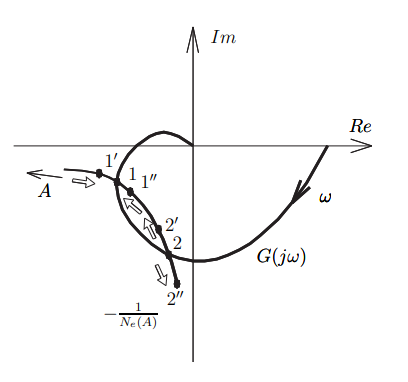
\includegraphics{img/stab.mez.cyklu.png}